%% ----------------------------------------------------------------------------
% BIWI SA/MA thesis template
%
% Created 09/29/2006 by Andreas Ess
% Extended 13/02/2009 by Jan Lesniak - jlesniak@vision.ee.ethz.ch
%% ----------------------------------------------------------------------------
\newpage
\chapter{Experiments and Results}
\label{sec:experimentsandresults}
\section{Training Models on MNIST, CIFAR and fastMRI}
In order to explore hyperparameters of the model architecture and debug the implementation, it was decided to first train models on datasets considered trainable with less computation time. Two very well known datasets in computer vision that use low-resolution images are CIFAR10 and MNIST.~\autocite{cifar,mnist}
\begin{figure}[h]
    \centering
    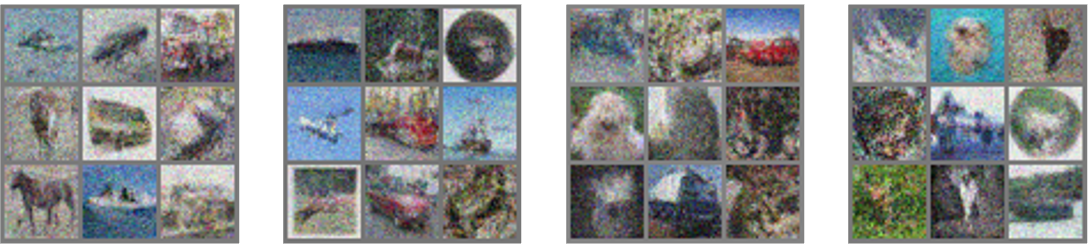
\includegraphics[width=.75\textwidth]{images/cifarsamples.png}
    \caption[Samples generated from CIFAR10]{Samples from the best performing model trained on CIFAR10 using a linear schedule: While the variance in the samples is large, suggesting that the model is able to capture the whole distribution, the samples are not completely denoised and therefore sample quality is seriously degenerated. As can be seen later, this was not observed when training on datasets where the image resolution was higher.}
    \label{fig:cifarsamples}
\end{figure}

\begin{figure}[h]
    \centering
    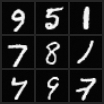
\includegraphics[width=.15\textwidth]{images/mnistsamples.png}
    \caption[Samples generated from MNIST]{Samples from the best performing model trained on MNIST.}
    \label{fig:mnistsamples}
\end{figure}

Unconditional sampling was performed in order to verify the sample quality and whether the model was able to capture the main modes of the training data distribution. For a quantitative analysis of sample quality and mode coverage/log-likelihood of trained models, Nichol et al. use FID score and log-likelihood estimates. FID requires an additional classifier network, which only makes sense on standardized datasets with class labels such as ImageNet or CIFAR~\autocite{imagenet, cifar}, where pretrained classifier weights are usually available, making scores comparable among different generative models. The fastMRI dataset is not meant for classification tasks, hence not containing any labels that could be used for such an evaluation. Getting robust estimates of the log-likelihood on the other hand requires evaluating the model on a significant portion of the training dataset, which was also omitted due to computational constraints. Instead, the diversity and quality of the samples was judged only visually and unconditional samples from 3 trained models can be seen in~\Cref{fig:cifarsamples,fig:mnistsamples,fig:uncondsampling}. All of those 3 models show good diversity among the samples, indicating good mode coverage, but while the perceptual quality of the samples is good for MNIST and fastMRI, the CIFAR10 samples are unsatisfactory. It might be more difficult to train DDPMs on resolutions significantly lower than $64\times 64$ as will be explored in the next section, and the only reason why the MNIST model managed to produce samples of high quality might be due to the comparative simplicity of the dataset.

The samples from Fig.~\ref{fig:uncondsampling} are sampled from a model trained on fastMRI RSS reconstruction at $128\times 128$ and that specific checkpoint was reached after 60 epochs or around 40'000 steps with a batch size of 48. This model carries the unique identifier \texttt{dutiful\-pond\-10} and was used for all subsequent experiments in the following sections. The exact hyperparameters are listed in Table~\ref{tab:dutifulpond10} and an overview over the training process is shown in Fig.~\ref{fig:dutifulpond10}. At this point it should be noted that subsequent reconstructions used images from the training set for guidance. Due to the high stochasticity of the DDPM and the very strong undersamplings that were used in this work, it is still a challenging problem to guide an unconditional DDPM to a good reconstruction of the input as will be demonstrated in the coming sections.
\begin{figure}[h]
    \centering
    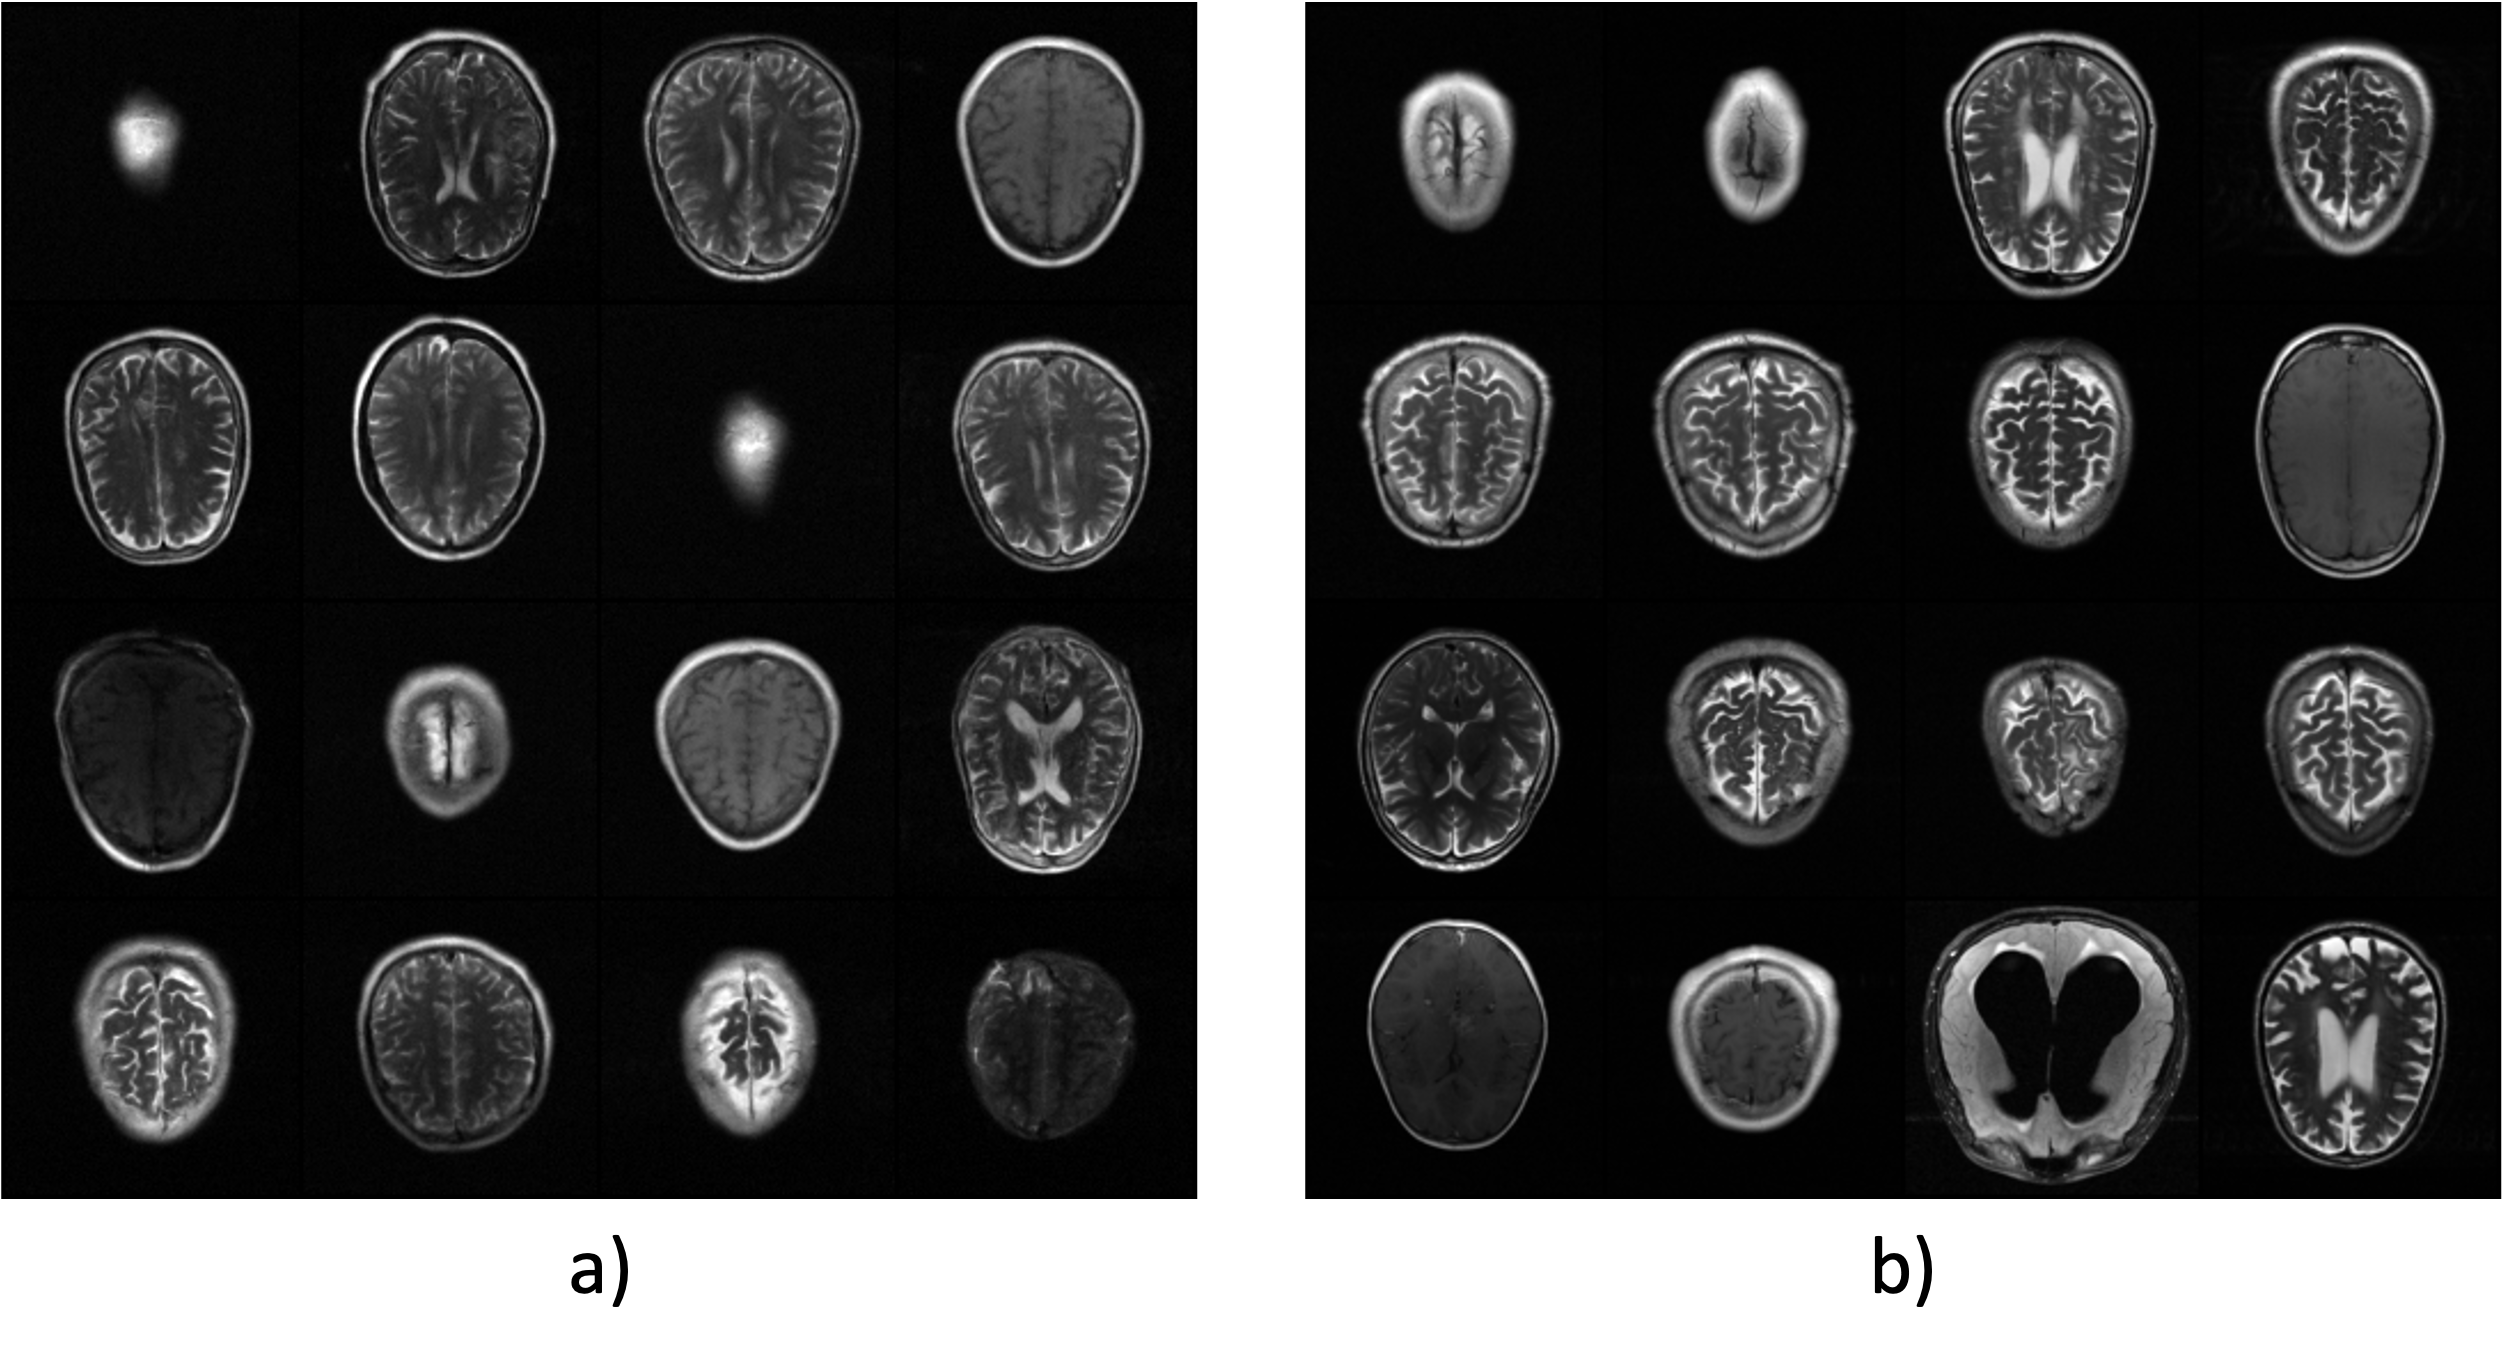
\includegraphics[width=.66\textwidth]{images/samples_unconditional.png}
    \caption[Samples from Data Set and Unconditional Sampling]{a) Unconditionally sampled examples, produced by the best-performing model \texttt{dutiful\-pond\-10}. b) Examples from the training data set (fastMRI, RSS reconstruction). As can be seen, sample quality is comparable to the quality of the training images and the variability among the samples is high, indicating a decent mode coverage of the model.}
    \label{fig:uncondsampling}
\end{figure}

\subsection{Influence of Schedules and Image Size on the Forward Diffusion}
\label{sec:forward_diff_experiments}
Ho et al. had derived a closed form solution to the forward process of DDPMs and Nichol et al. investigated alternative options for the noise scheduling.~\autocite{ho2020denoising,nichol2021improved} They concluded that the important parameters to model are not the variances $\beta$ of the transitions, but the variances $1-\bar{\alpha}$ of the closed-form forward process, since they are the ones responsible for the destruction of information.

They decided to use a squared cosine function for the $1-\bar{\alpha}$, since this would be close to linear in the middle and would smoothly transition to constants towards the critical beginning and end points of the process. Fig.\ref{fig:alphadash} shows how $1-\bar{\alpha}$ and $\beta$ behave for the two approaches of either modeling the $\beta$ linearly, or modeling the $1-\bar{\alpha}$ according to a squared cosine. It is immediately visible that the variances of the linear schedule reach the maximum too early and flatten out, leading to the intuition that the last few steps are not very useful.

\begin{figure}[h]
    \centering
    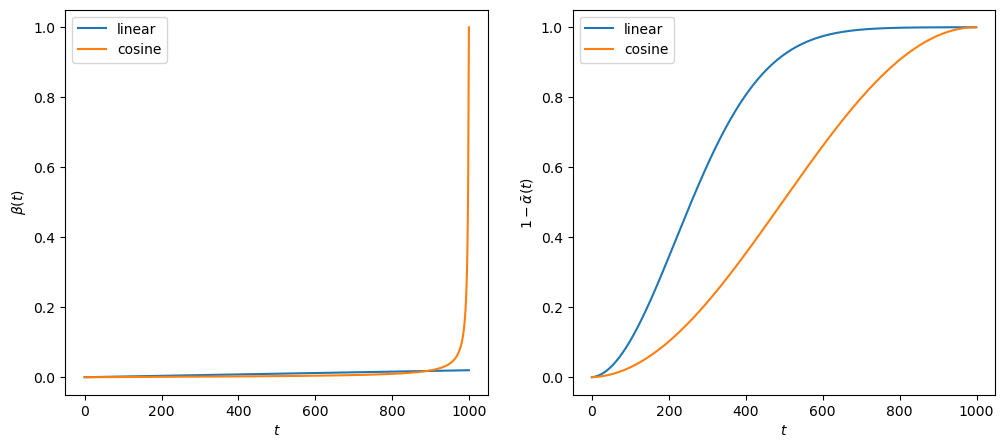
\includegraphics[width=.7\textwidth]{images/variance_schedule_alphadash.png}
    \caption{Variance Schedule Approaches: Modeling the $1-\bar{\alpha}$ as an approximate linear function (right cosine) and deriving $\beta$ (left cosine), or modeling $\beta$ as a linear function (left linear) and deriving $1-\bar{\alpha}$.}
    \label{fig:alphadash}
\end{figure}

The intution can experimentally confirmed by measuring how closely the latent representations go to isotropic noise when passing samples through the forward process. For this a batch of 50 times the same image $x_0$ was passed through the forward process and the covariance matrix over all $x_T$ was calculated. As a metric for how close the covariance matrix was to the identity covariance matrix of pure i.i.d Gaussian noise, the identity matrix was subtracted and the mean of the absolute value of the matrix calculated. The experiment was conducted at several image resolutions, since Nichol et al. found the cosine schedule to be superior mainly for low resolution images. The results can be seen in Fig.~\ref{fig:noisecloseness} and confirm the intuition: When using linear scheduling the closest point to pure noise is already reached after around 600 steps for small images, and after around 700 for larger images. Even more interesting is the fact that both schedules struggle to reach pure noise for the lowest two resolutions, which might be a reason for the poor sample quality reached on the CIFAR10 dataset, that was shown in the previous section.

\begin{figure}[h]
    \centering
    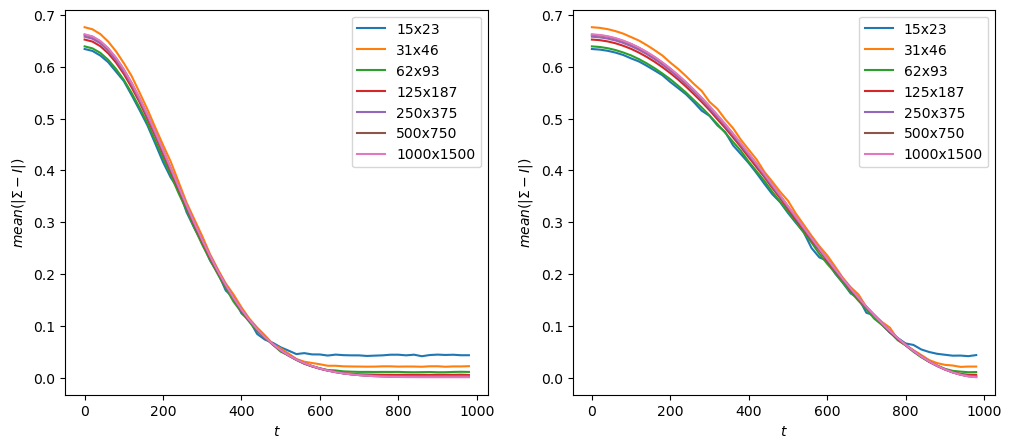
\includegraphics[width=.7\textwidth]{images/frobenius_norm.png}
    \caption{Closeness to i.i.d Gaussian noise for linear scheduling (left) and cosine scheduling (right).}
    \label{fig:noisecloseness}
\end{figure}

\section{Image Inpainting \& Low-Frequency Guidance}
The works by Lugmayr et al.~\autocite{lugmayr2022repaint} and Choi et al.~\autocite{choi2021ilvr} were the primary motivation behind pursuing an approach of conditioning unconditionally trained DDPMs. As a first step it was therefore important to recreate their results before adapting them to the task of undersampled MRI. The update steps of the reverse diffusion process were formulated according to the formulas from section~\ref{sec:freqreplacement} and the results can be seen in Fig.~\ref{fig:repaint} and Fig.~\ref{fig:ilvr} for RePaint and ILVR respectively.

Using Lugmayr et al.'s suggested hyperparameters for resampling (jump length of 10, with 10 resamplings) was indeed observed to help with creating semantically meaningful reconstructions~\autocite{lugmayr2022repaint}, with the exception of a single sample (lowest row, second from left). This specific sample also caused issues with ILVR, indicating that the distributional mode of that image type was not learned well by the model. Since it is an unusual type of image, it was likely not represented well in the training data.

\begin{figure}[h]
    \centering
    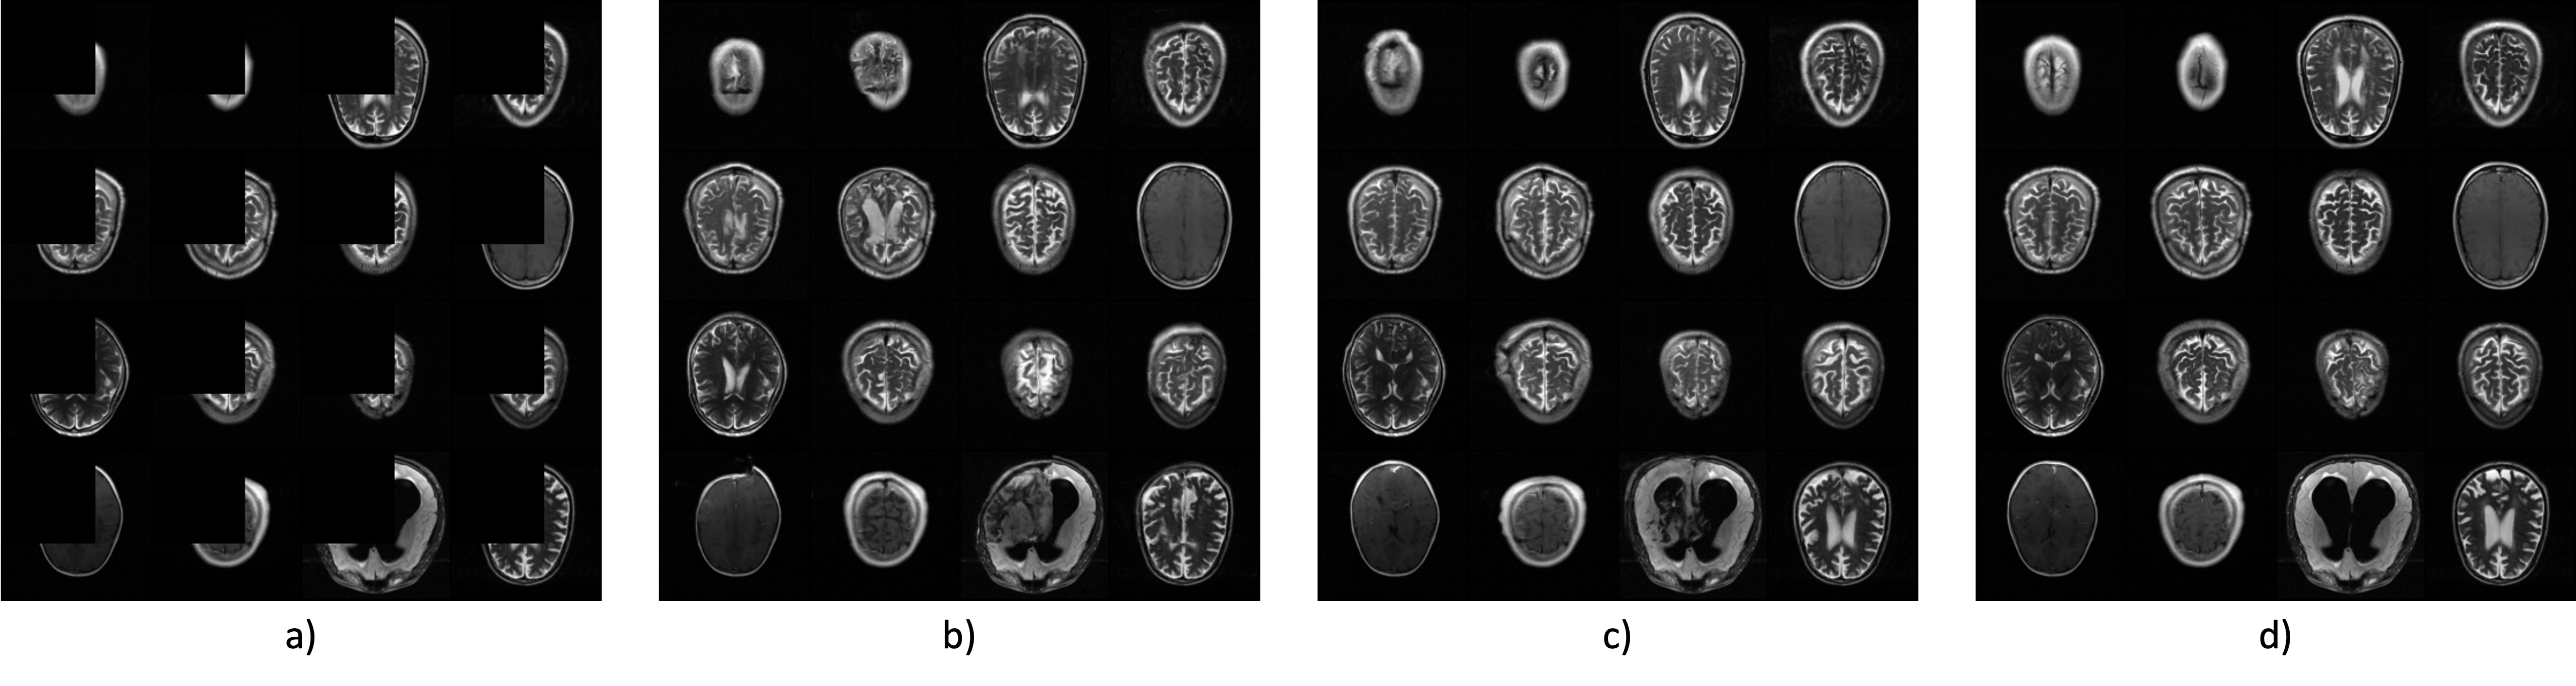
\includegraphics[width=.8\textwidth]{images/repaint.png}
    \caption[Inpainting and Resampling]{Inpainting and Resampling: a) Masked images used for the RePaint-style conditioning of the unconditional DDPM. b) Results from direct sampling. The reconstructed areas are often semantically wrong. c) Results from sampling with resampling with jump length $j=10$ and resamplings $r=10$ as suggested by Lugmayrs et al~\autocite{lugmayr2022repaint}. As observed in their work, the resampling strategy helps with semantically meaningful reconstruction. d) Ground truth images for comparison.}
    \label{fig:repaint}
\end{figure}

While Choi et al. used a linear filter consisting of downsampling and upsampling operations, the filter used in this work was a Gaussian kernel. As can be seen in the samples of Fig.~\ref{fig:ilvr}, the model produces final images that match the rough shape of the guidance examples, but often differ substantially in the details. In many instances the type of the final image is not even the same as the guidance type. As would be expected, this was not observed when using less blurry images for the guidance.

\begin{figure}[h]
    \centering
    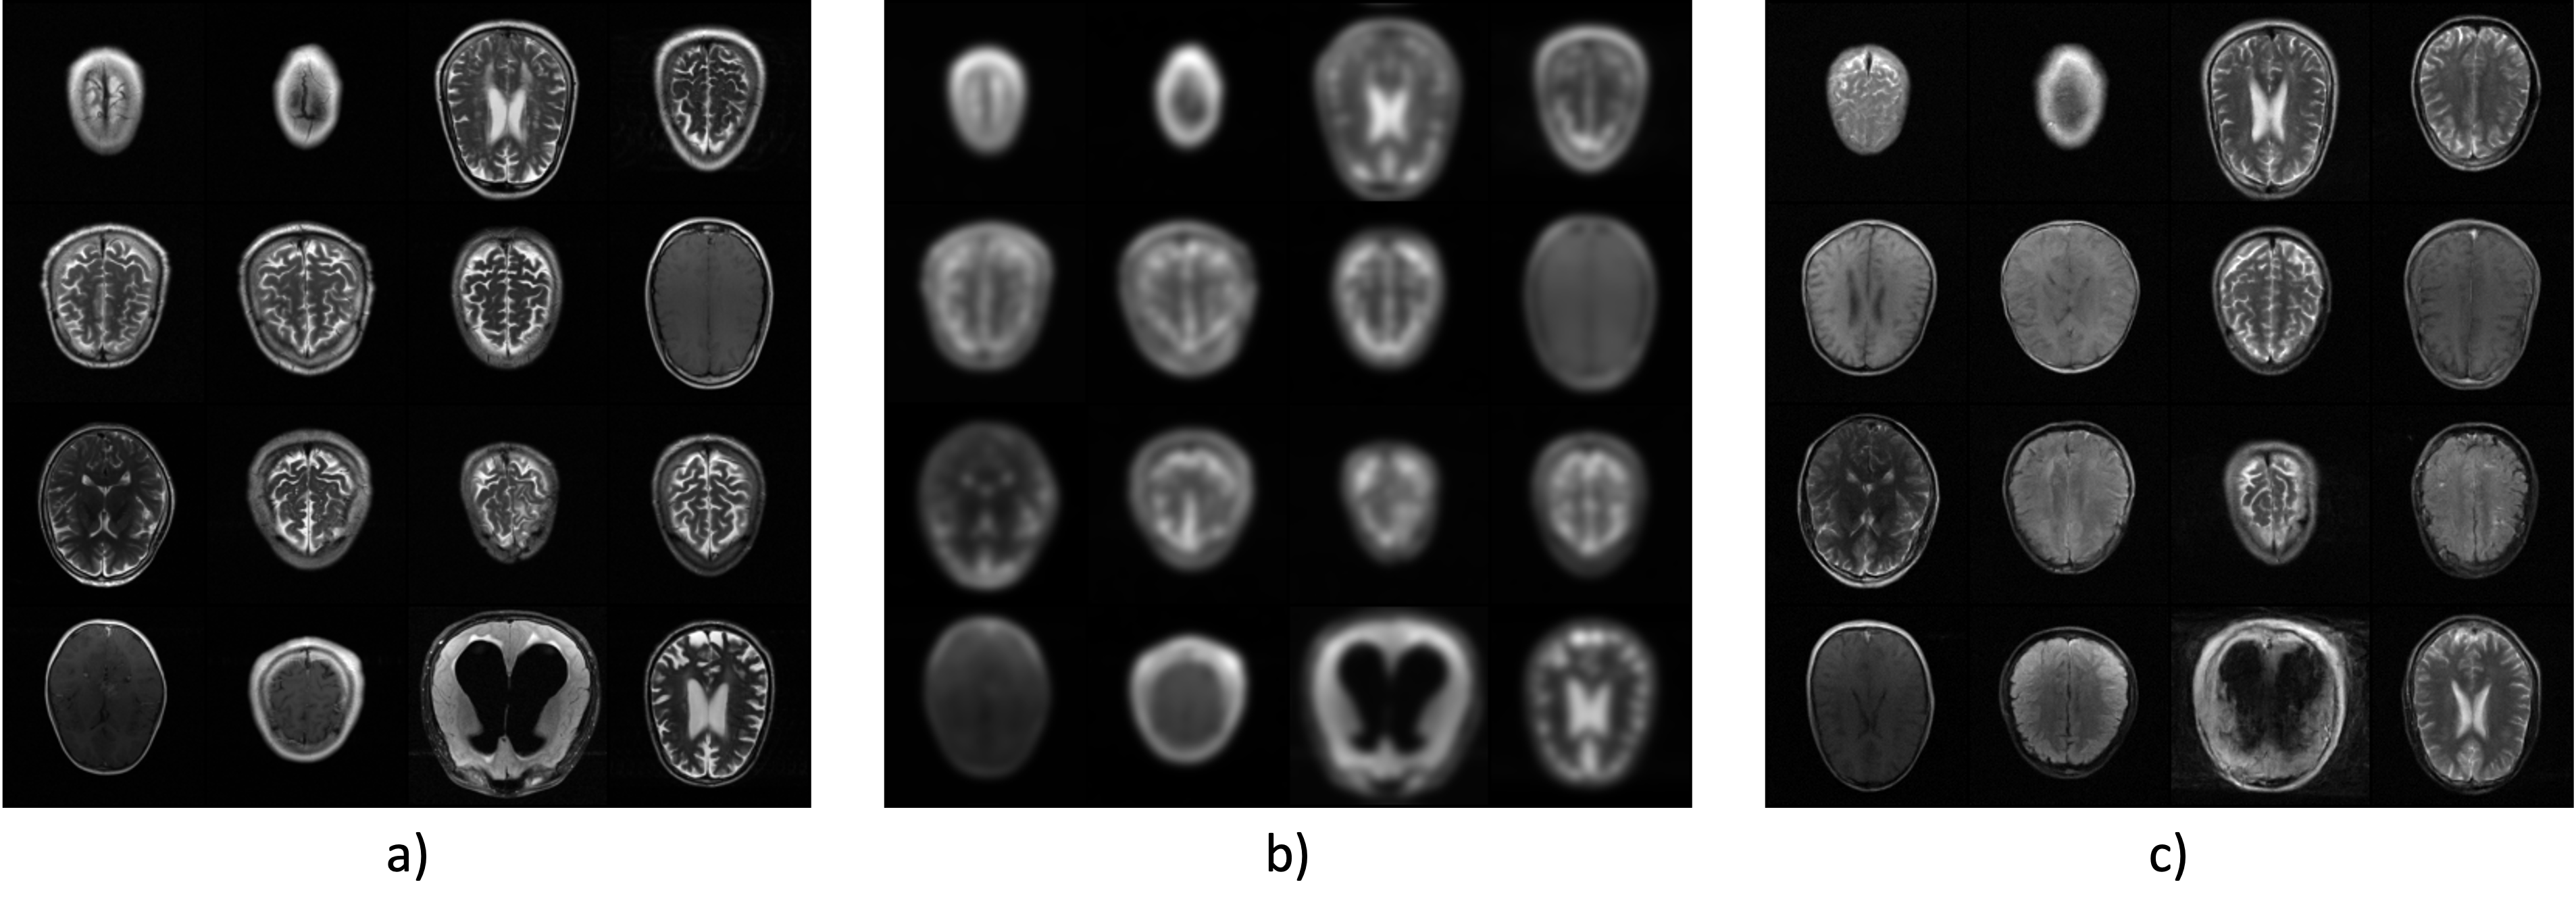
\includegraphics[width=.6\textwidth]{images/ilvr.png}
    \caption[ILVR -- Low-Frequency Guidance]{ILVR -- Low-Frequency Guidance: a) Original guidance images. b) Filtered version used for guidance. c) Final predictions using the filtered guidance images. As can be seen, the predictions are of good perceptual quality, but the predictions often do not match the ground truth images, indicating that the filtering was too strong in this specific case.}
    \label{fig:ilvr}
\end{figure}

\section{Masked K-Space Substitution}
As introduced in section~\ref{sec:freqreplacement}, ILVR and RePaint can be used to replace parts of k-space in the prediction according to
\begin{equation}
    \label{eq:kspacesubstituion}
    x_{t-1} = x_t - \mathcal{F}^{-1}\left(\mathcal{M}\circ\mathcal{F}(x_t) + \mathcal{M}(s_t)\right)
\end{equation}
with $\mathcal{M}$ being a masking operation and $s_t$ being the latent representation of the known k-space. The latent $s_t$ can be derived from $s_0$ by applying noise either in the image space or directly in k-space and results using both techniques for MRI reconstruction are depicted in Fig.~\ref{fig:freqreplacement}. The sample quality is significantly worse than for ILVR or RePaint, which is surprising since a relatively low acceleration of factor $\approx 4.12$ was used. The samples suffer from noticeable aliasing artifacts and unsharp edges, which might stem from the model being guided into the wrong ditributional mode and the fact that k-space masks are multiple passband box filters that could induce ringing artifacts. Aliasing and ringing are usually avoided by using filters and the simplest choice of filter that avoids such artifacts is a Gaussian kernel. Gaussian filters are also linear filters, which means that they integrate well into the framework from Eq.~\ref{eq:kspacesubstituion}. The downside of applying a Gaussian filter are twofold: 1. Discarding higher frequencies would be wasteful, since they consumed acquisition time; 2. The results from ILVR showed that low frequency guidance can guide the model to a different distributional mode than the target image, which indicates that the high frequencies are not only important for matching the smallest details. The next section will explore the idea of adding information gradually over the reverse diffusion process, making higher frequencies available to the model, but only towards the end of the process. Since this allows the use of smooth filters like a Gaussian, it was hypothesized to partially solve the issues of unsharp edges and aliasing.

RePaint-style resampling was mainly developed to help with matching semantics therefore it was not expected to yield similar performance improvements for MRI reconstruction. Nevertheless, the resampling technique was also used together with the update step from Eq.~\ref{eq:kspacesubstituion} in order to see if sample quality can be improved through increased computation time, but this was not the case.
\begin{figure}
    \centering
    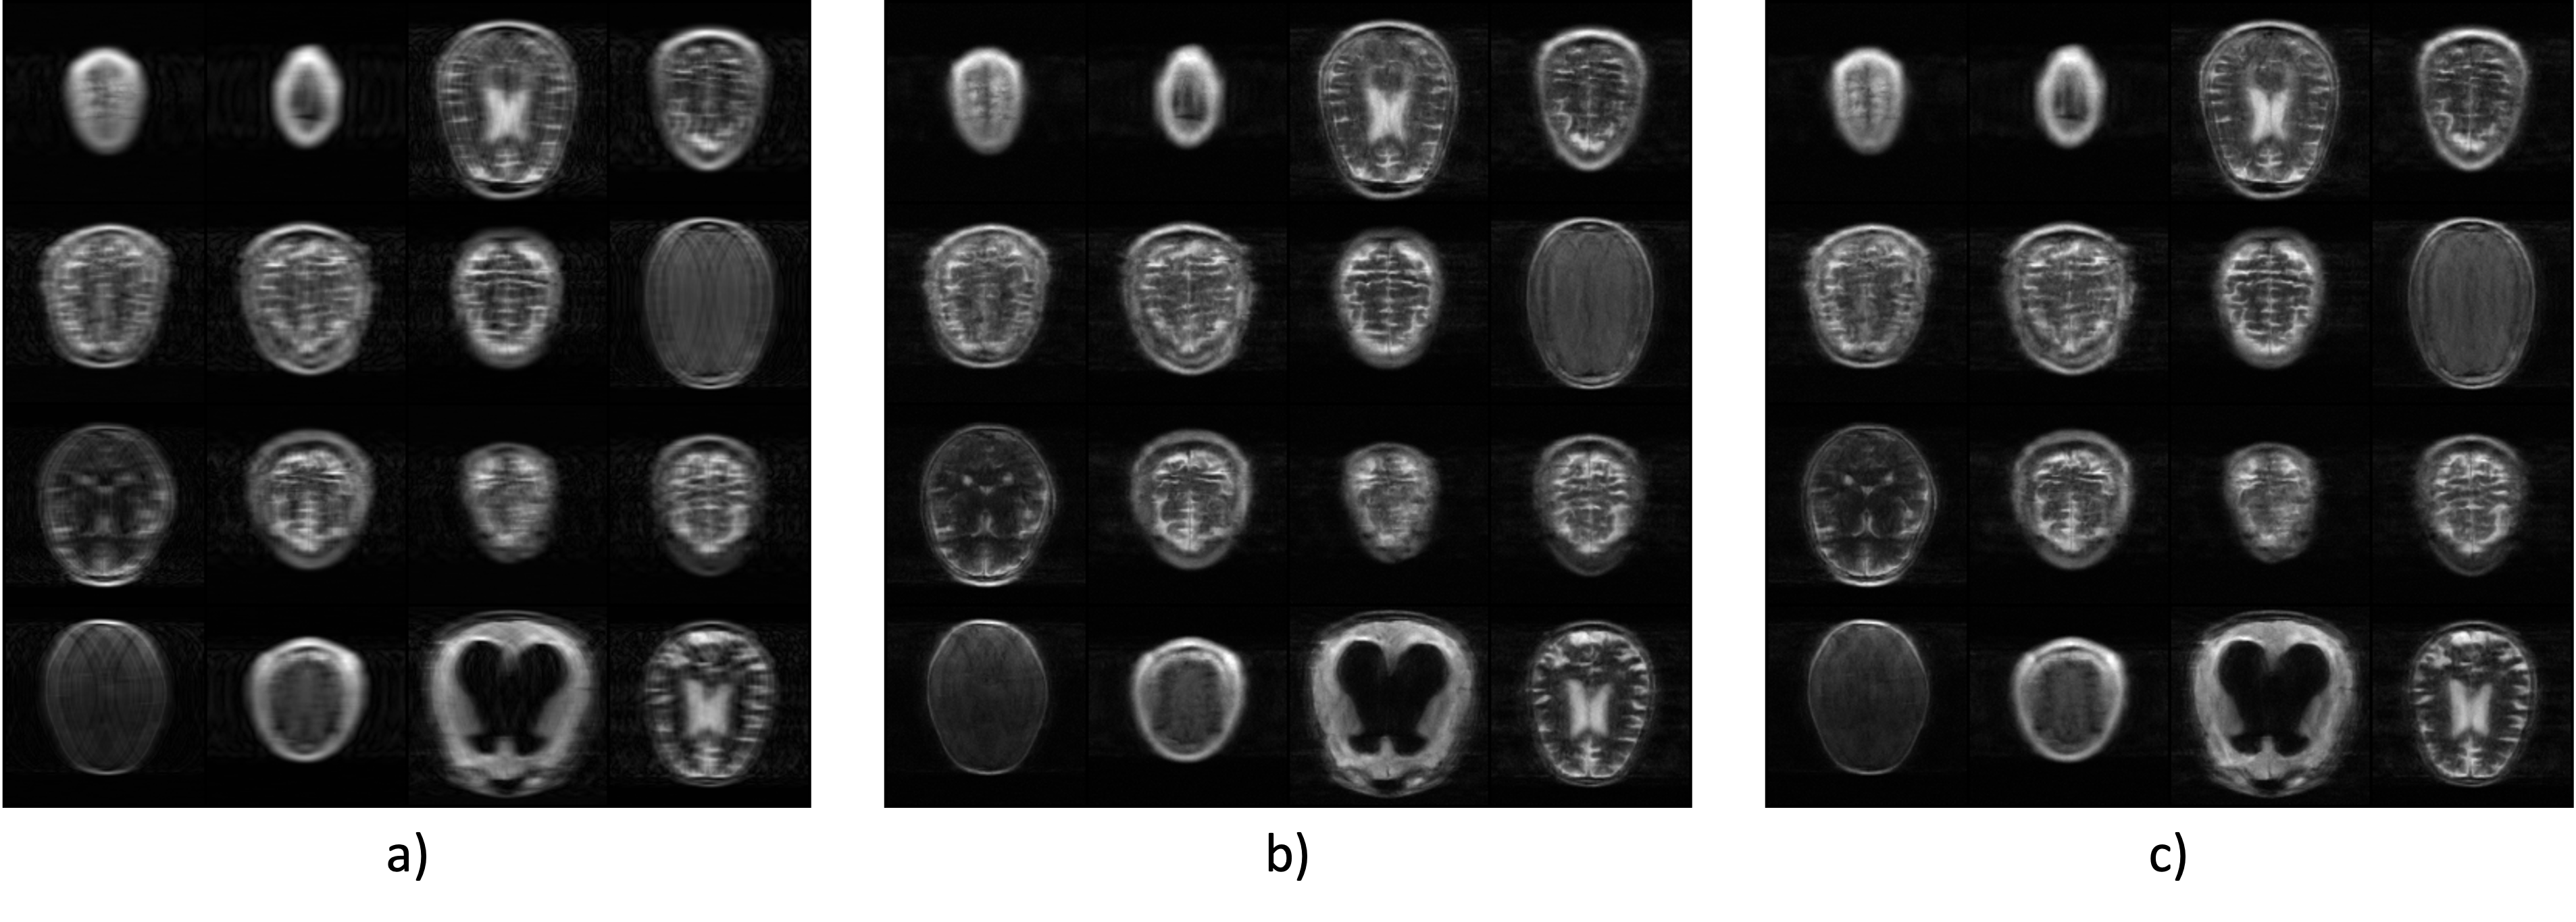
\includegraphics[width=.6\textwidth]{images/freq_replacement.png}
    \caption[Frequency Replacement]{Diffusion guidance using frequency replacement: a) Corrupted samples from an acceleration $\approx 4.12$. b) Results from applying noise directly on k-space (see~\ref{sec:freqreplacement}). c) Results from applying noise in the image space. The reconstruction quality is similar in both cases, but significantly worse than experiments with RePaint and ILVR from the previous section would suggest. The reconstructions show aliasing artifacts and possibly ringing artifacts at the edges, which indicate serious frequency mismatch.}
    \label{fig:freqreplacement}
\end{figure}


\section{Variance in Predictions and Filtered Diffusion}
\label{sec:predvariance}
Since the SNR (signal-to-noise-ratio) in natural images is much higher in the lower frequencies than in the higher ones, it was hypothesized that higher frequencies carry very little information early in the reverse diffusion process and it might therefore be possible to add frequency information gradually during the denoising process. Lower frequencies first to provide more broad information and higher frequencies only at the end to make sure that the details of the image match. Since this could be done by applying filters of varying pass bands, it might partially solve the issues of aliasing and ringing.

In order to empirically study the relevance of the frequencies, a single sample was denoised and its latent representations at every 10th timestep were saved. These latent representations were copied into batches of 100 equal latent representations and the denoising process was continued for all these batches. Fig.~\ref{fig:predvariance} shows 4 of these samples for a subset of starting points. As can be seen, when starting from $t\geq700$, the samples still have a lot of variability and share very few common features. When starting later in the process, the samples clearly stem from the same distributional mode and only differ in the details. Since high frequencies are responsible for carrying information on details, this supports the hypothesis, but it becomes more evident, when looking at the variances of the spectral representations as seen in Fig.~\ref{fig:spectralvariance}. The variances were estimated over the frequency representations of all the final predictions in a batch (100 samples, denoised from a starting point $t$) and high variance in a frequency indicates that the value of this frequency was not yet determined at starting point $t$. As can be clearly seen in the figure, the variance is concentrated in the low frequencies when starting from a large $t$ and the variance of the low frequencies only becomes comparable to it when starting late in the process (small $t$). This again supports the hypothesis that high frequencies matter much more towards the end and that it might be possible to only introduce them later in the process.
\begin{figure}[h]
    \centering
    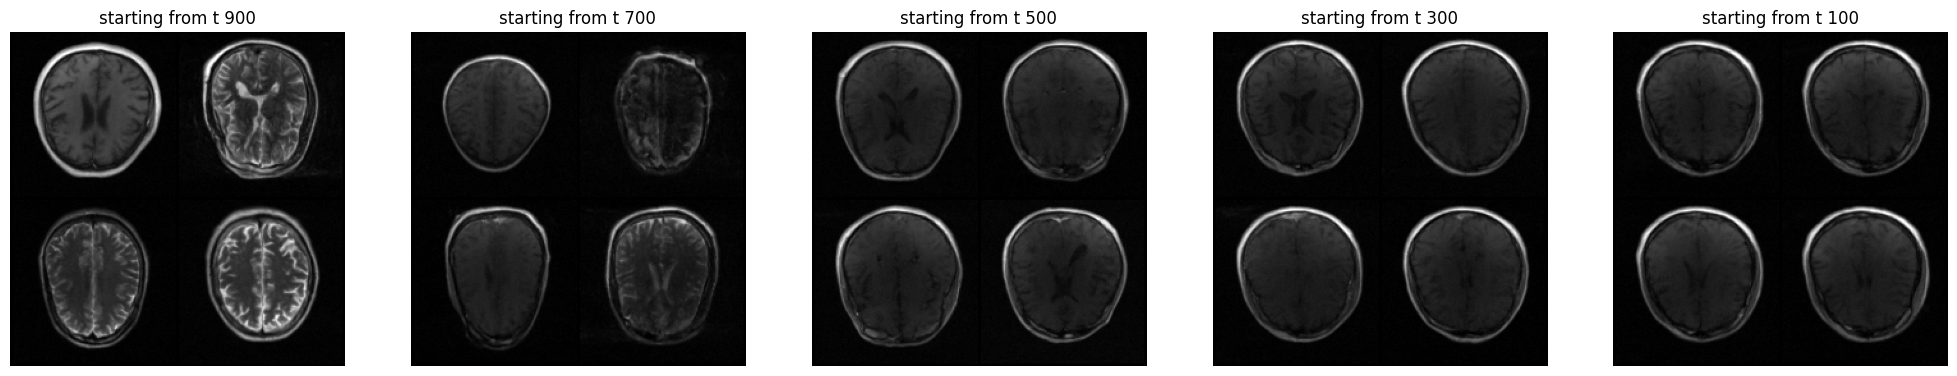
\includegraphics[width=\textwidth]{images/fixedlatents_variance.png}
    \caption[Variance in Predictions from Fixed Latents]{Variance in Predictions from Fixed Latents: The general shape of the final samples is already determined at $t=500$ and from there, the variability in the outputs is mostly about details of the structure.}
    \label{fig:predvariance}
\end{figure}

\begin{figure}[h]
    \centering
    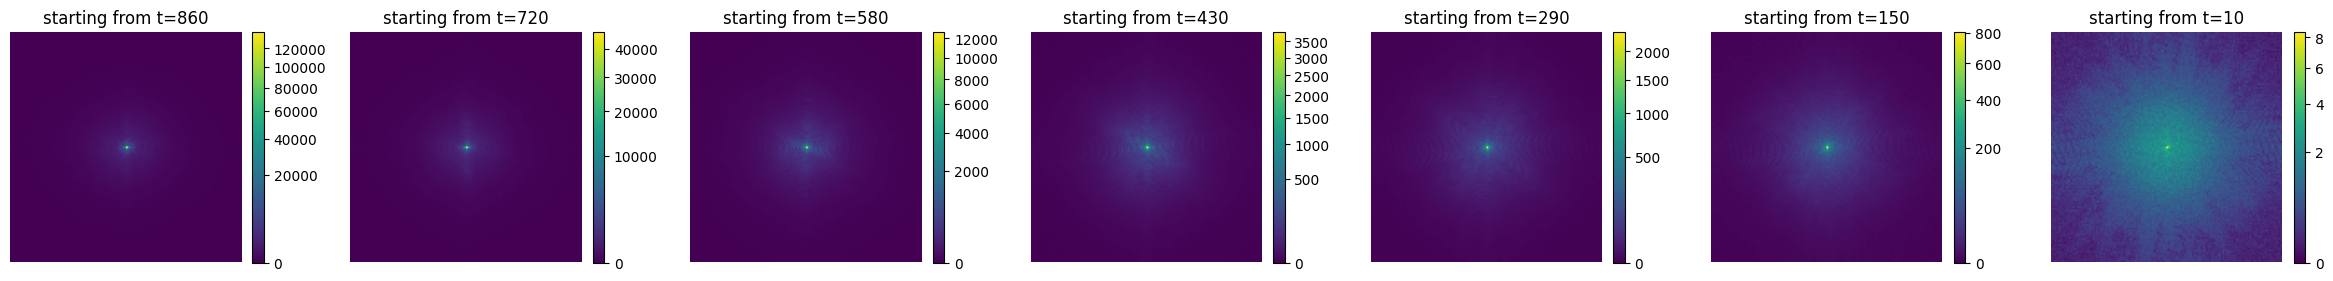
\includegraphics[width=\textwidth]{images/fixedlatents_varSpectra.png}
    \caption[Spectral Variance from Fixed Latents]{Variance in the Spectra when starting from Fixed Latents: When generating samples from fixed latent representation early in the denoising process, the variance of the spatial frequencies is highly concentrated in the center (e.g. $t=860$), overpowering the variance in the low frequencies by several orders of magnitude. The differences are smaller when starting late in the process (e.g. $t=10$), suggesting that fine details are only reconstructed at the very end. This hypothesis is also supported by the fact that natural images have lower SNR in the higher frequencies, which means that Gaussian perturbation affects them more and they can't carry much information until most of the noise is removed.}
    \label{fig:spectralvariance}
\end{figure}

A gradual introduction of frequencies could be done by introducing a schedule of k-space masks, but this would again equate to box filters, which should be avoided for the reasons mentioned in the previous section. Instead, a schedule of standard deviations for the 1D Gaussian filter was used and the time dependent filter ($\phi \rightarrow \phi(t)$) was added to Eq.~\ref{eq:kspacesubstituion} as
\begin{equation}
    x_{t-1} = x_t - \mathcal{F}^{-1}\left(\phi(t)\circ\mathcal{M}\circ\mathcal{F}(x_t) + \phi(t)\circ\mathcal{M}(s_t)\right).
\end{equation}
Results with such scheduled filters were in general unsatisfying with some samples showing a slight improvement over unfiltered frequency replacement, while in others, the aliasing issue was actually amplified, as demonstrated in Fig.~\ref{fig:filtereddiffusion}. The search space over different schedules that could improve the outcome is very large and since loss guidance (\ref{sec:lossguidance}) had been identified as a very flexible and powerful approach at this point, optimization of the scheduling or resampling strategies using filter schedules were not further investigated. Loss guidance also offered another possibility of inspecting dominant frequencies in the guidance process and the results of this experiment are shown in Fig.~\ref{fig:lossgradients}.
\begin{figure}
    \centering
    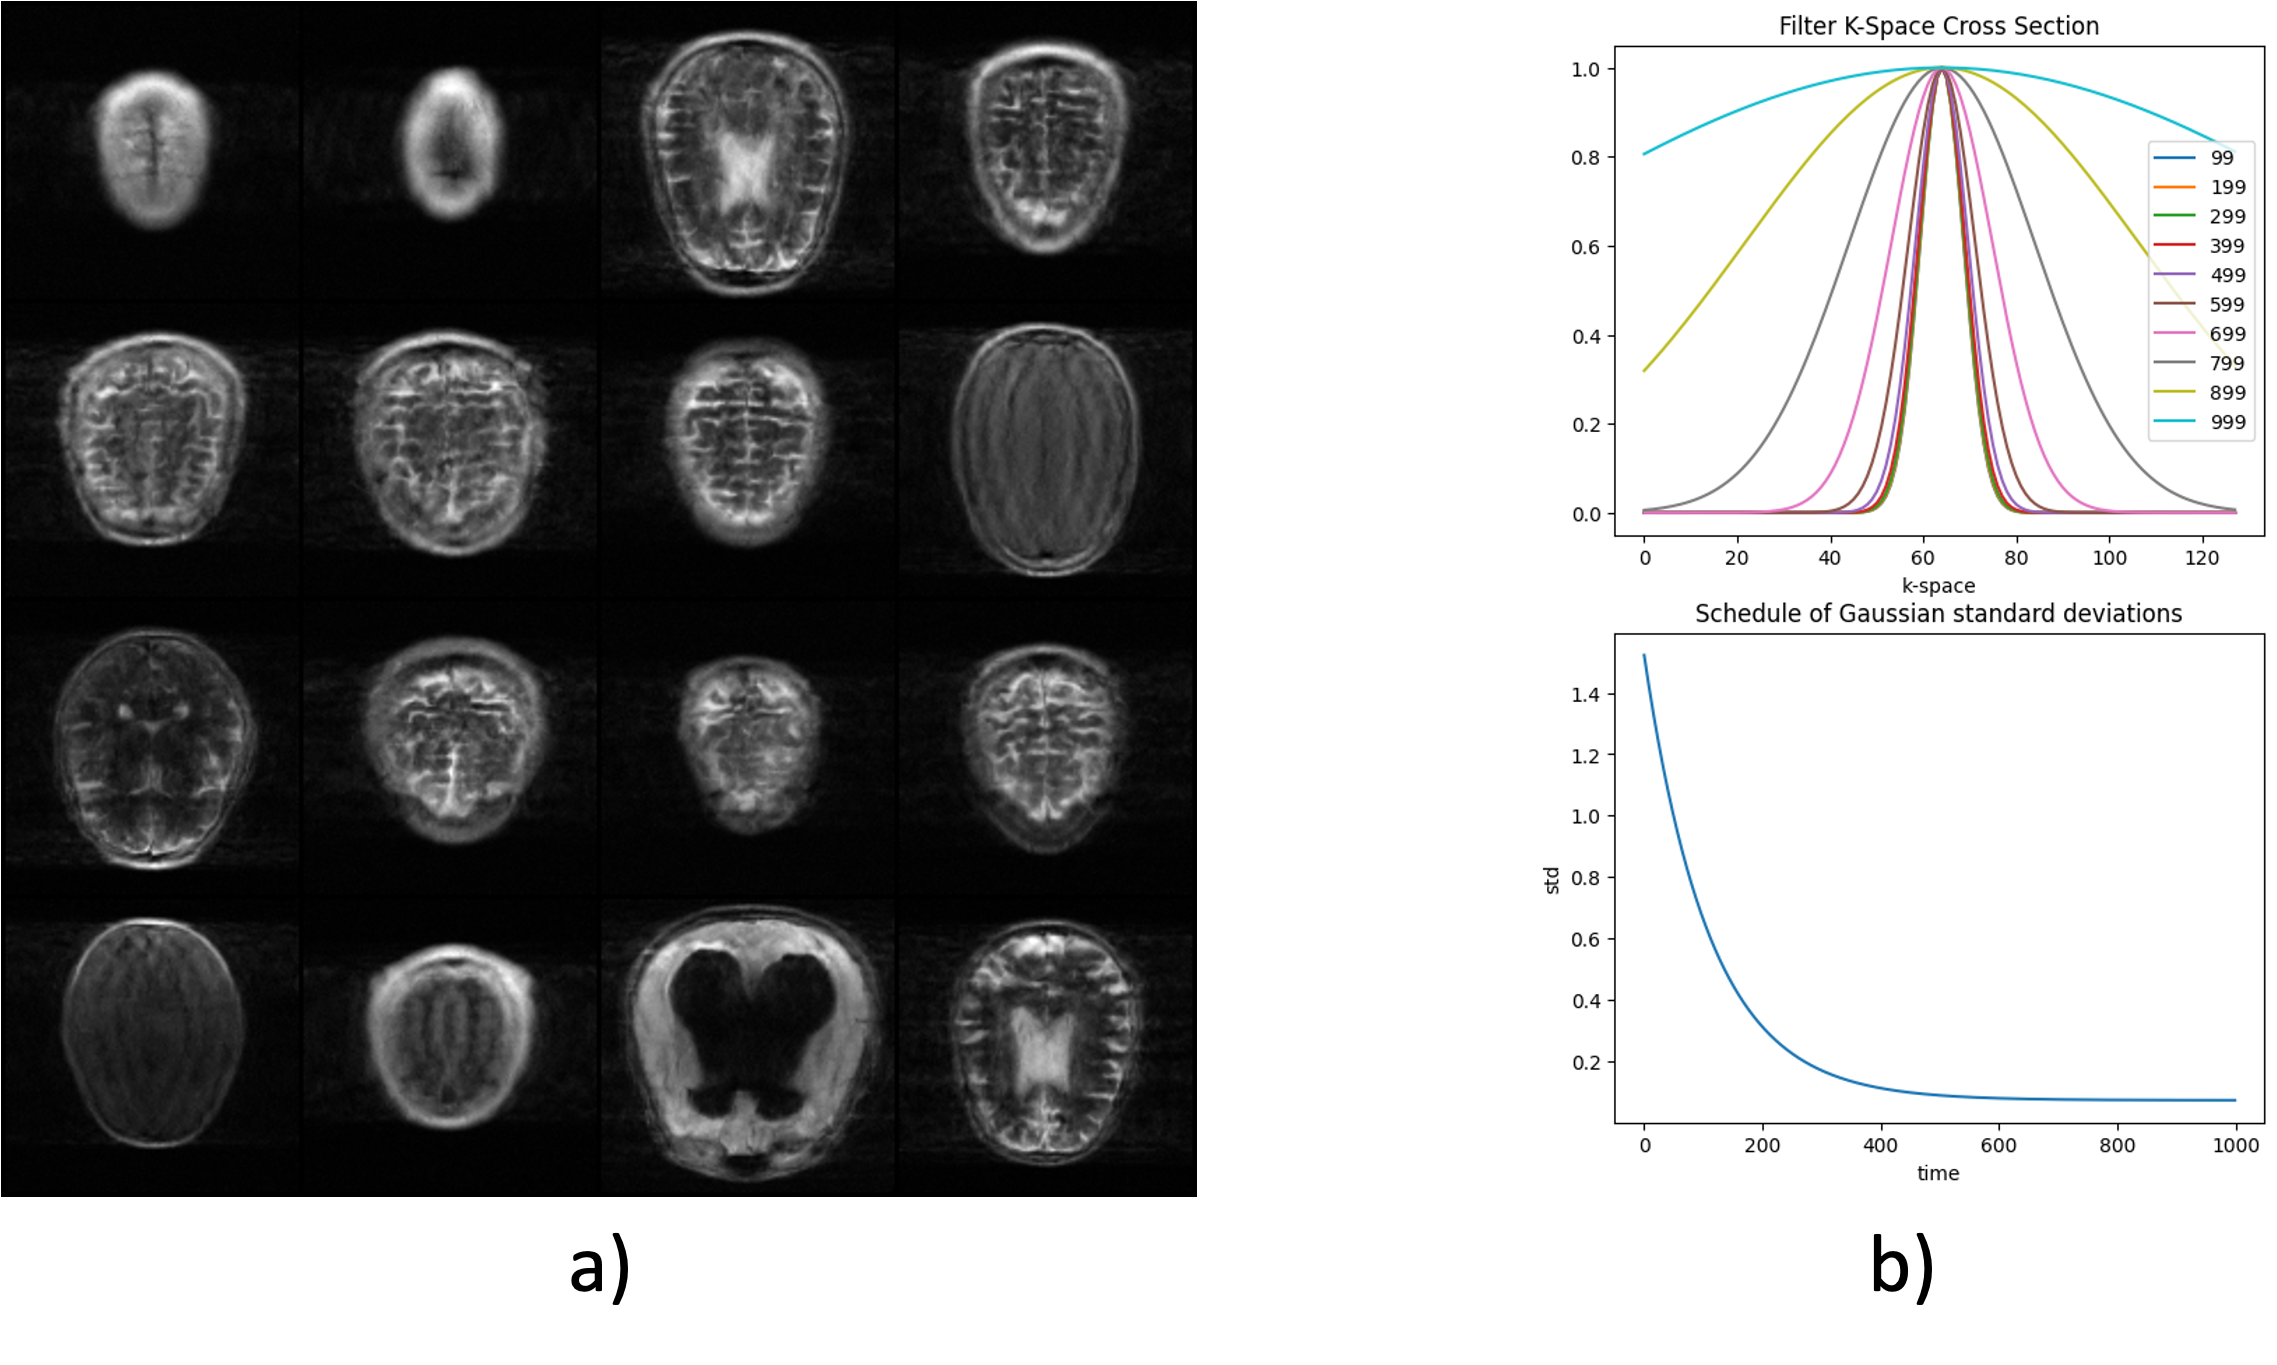
\includegraphics[width=.7\textwidth]{images/filtereddiffusion.png}
    \caption[short]{Results from scheduled filtering: a) Results from using Gaussian filters during reverse diffusion, scheduled according to the standard deviations in b) (lower). While contrast is in general enhanced compared to simple frequency replacement, and some samples show better perceptual quality, aliasing is amplified for others. While this was not further investigated, it may be that those samples were initially guided into a wrong distributional mode in which later introduced frequencies matched even worse.}
    \label{fig:filtereddiffusion}
\end{figure}

\section{Loss Function Guidance}
\subsection{Direct Sampling}
Taking gradient steps in the direction of a loss gradient immediately proved to be a more flexible approach with much better reconstruction results than the previous methods. Since PyTorch's auto-differentiation can not only calculate gradients with respect to weights, but also with respect to inputs, the calculation of the loss gradients was simple to implement as can be seen in Listing~\ref{lst:lossgradient}. Since prediction and ground truth k-space are masked, the loss is only influenced by the known areas, which is why it needs to be scaled by the acceleration. Otherwise loss values are not comparable between different acceleration masks and suitable guidance factors would have to be derived individually for every mask. As mentioned in~\ref{sec:lossguidance}, this approach would naturally extend to other types of loss functions like $\text{L}_1$ and MSE was chosen for the similarity between its gradient and the replacement strategy (section~\ref{sec:freqreplacement}).
\begin{lstlisting}[language=iPython, caption=Calculation of the loss gradient., float=htbp, label=lst:lossgradient]
    def mse_grad(pred: Tensor, corrupted_kspace: Tensor, mask: Tensor) -> Tuple:
        pred = pred.requires_grad_(requires_grad=True)

        # corrupted_kspace is already masked
        pred_masked_kspace = to_kspace(pred) * mask
        loss = mse_loss(pred_masked_kspace, corrupted_kspace)

        # loss scaling for different masks
        eff_acc = torch.mean(mask.view(-1))
        loss = loss / eff_acc

        grads = torch.autograd.grad(loss, pred)[0]
        pred = pred.requires_grad_(requires_grad=False)

        return grads, loss.item()
\end{lstlisting}
Results that use loss guidance for the reconstruction can be seen in Fig.~\ref{fig:reconstructionslossguidance} and they are of very high quality for the lower accelerations of $3.12$ and $5.57$, but drop when speeding up acquisition by a factor of $11.64$. The magnitude of the guidance factor is responsible for balancing the prior and the data consistency, and this is especially visible for the highest acceleration, where samples guided by $g=20'000$ have much higher perceptual quality than samples guided by $g=200'000$. A broader view on the tradeoff between sample fidelity and data consistency can be viewed in Fig.~\ref{fig:directsamplingcomparison}, where a larger range of guidance factors is considered and the tradeoff becomes more evident. For very low guidance factors ($\approx 1000$), it can further be observed that the samples lack contrast. Similar observations were made by Dhwariwal et al., where classifier guidance yielded signficantly improved contrast over unconditional sampling.~\autocite{dhariwal2021diffusion}
\begin{figure}
    \centering
    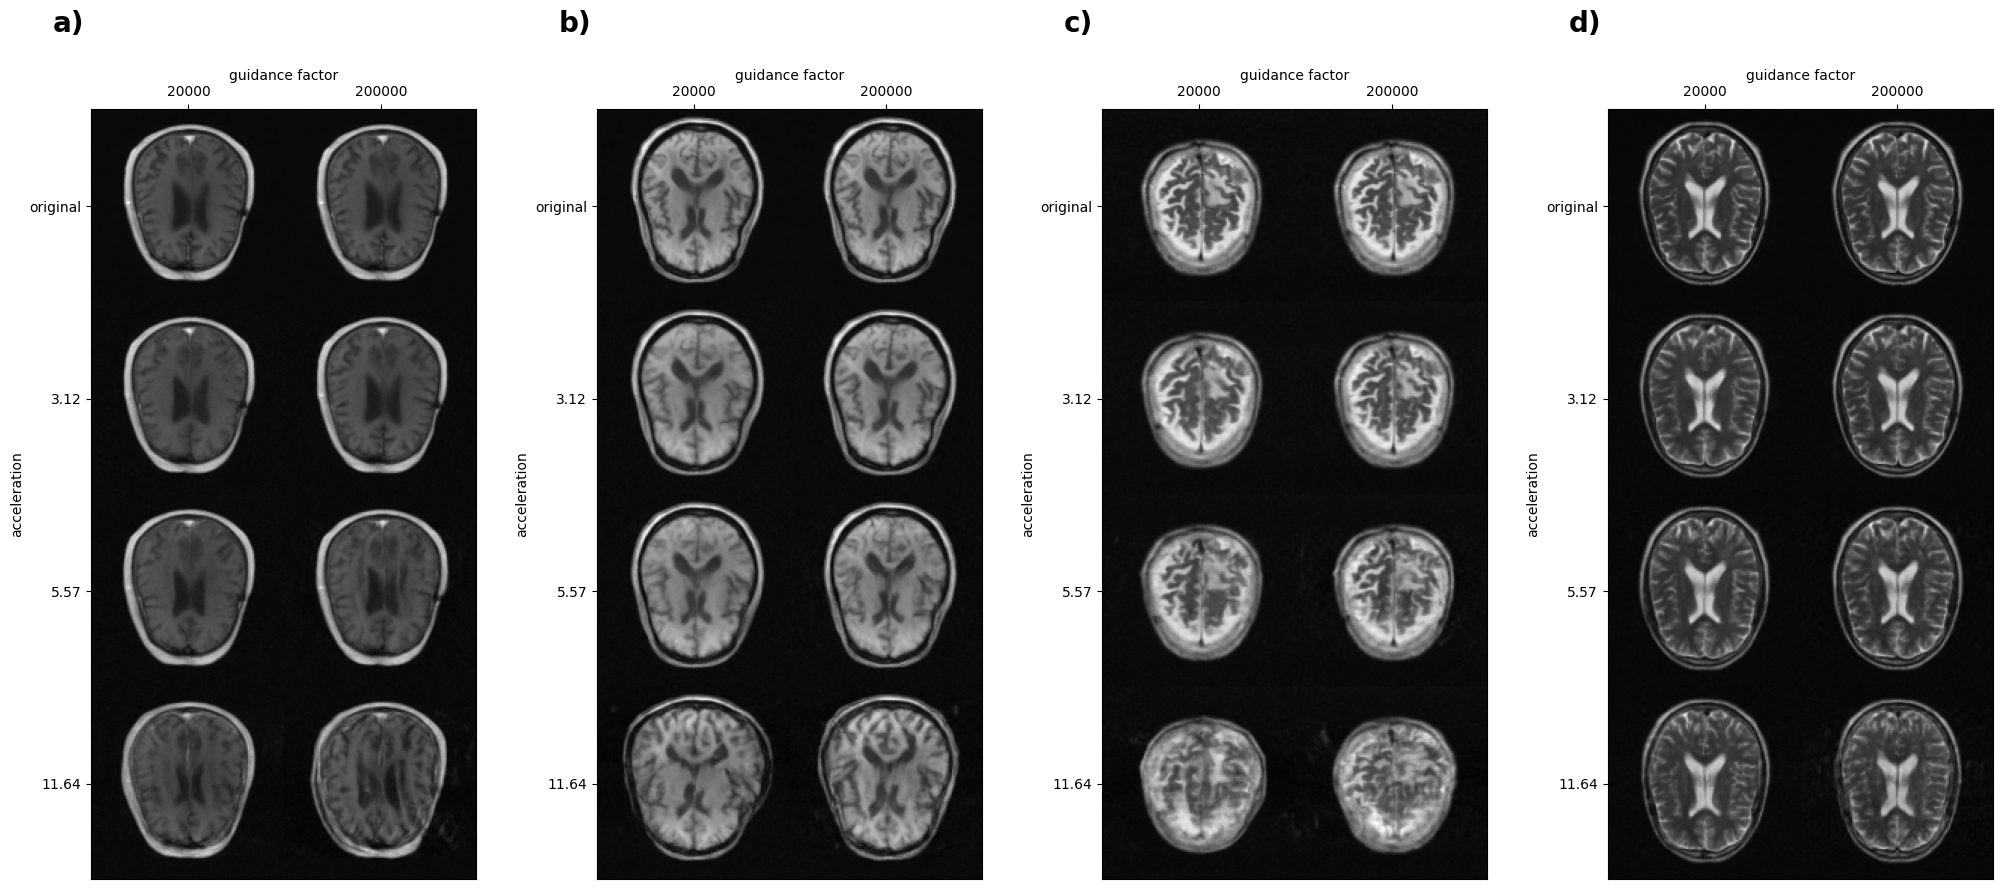
\includegraphics[width=\textwidth]{images/directsampling_small.png}
    \caption[Reconstructions using Loss Guidance]{Reconstructions using Loss Guidance: a) - d) Reconstructions for three different accelerations and two different guidance factors. The quality of the reconstructions is usually good for the two lower accelerations, but drops significantly for the very high acceleration of $11.64$. The reconstructions with the highest acceleration also show how the guidance factor can be used to trade off data consistency for sample quality, with the lower guidance yielding visually pleasing images with fewer artifacts.}
    \label{fig:reconstructionslossguidance}
\end{figure}

In order to evaluate the reconstruction quality empirically, the mean squared error to the ground truth was calculated and the results for different accelerations can be seen in Fig.~\ref{fig:lossguidancelosses} a), where the results were averaged over 100 different samples. For the lower accelerations, the MSE continually decreased with increasing guidance and no point was reached where guidance allocated too much weight to the data consistency. For the highest acceleration, the loss essentially stops decreasing at $g=50'000$, with slight fluctuations in the losses for higher guidance values. This fits the observations from Fig.~\ref{fig:reconstructionslossguidance} and Fig.~\ref{fig:directsamplingcomparison}, where higher guidance values usually led to aliasing. Fig.~\ref{fig:lossguidancelosses} b) - d) also includes plots of the running losses for the different accelerations and guidance factors. In contrast to the final MSE, this running loss is calculated in k-space and is weighted by the mask coverage (see Listing~\ref{lst:lossgradient}). While it is unsurprising that higher guidance leads to a faster decrease of the MSE, it is counterintuitive at first that the losses decrease faster for the highest acceleration, since it provides less guidance information. The explanation likely lies in the fact that high acceleration masks sample mainly in low frequencies and the loss is therefore concentrated in the center of k-space. As discussed in~\ref{sec:predvariance}, low frequencies have higher SNR and having only those available early for guidance might lead to less noisy gradients early in the reverse diffusion process and subsequent faster convergence.
\begin{figure}[h]
    \centering
    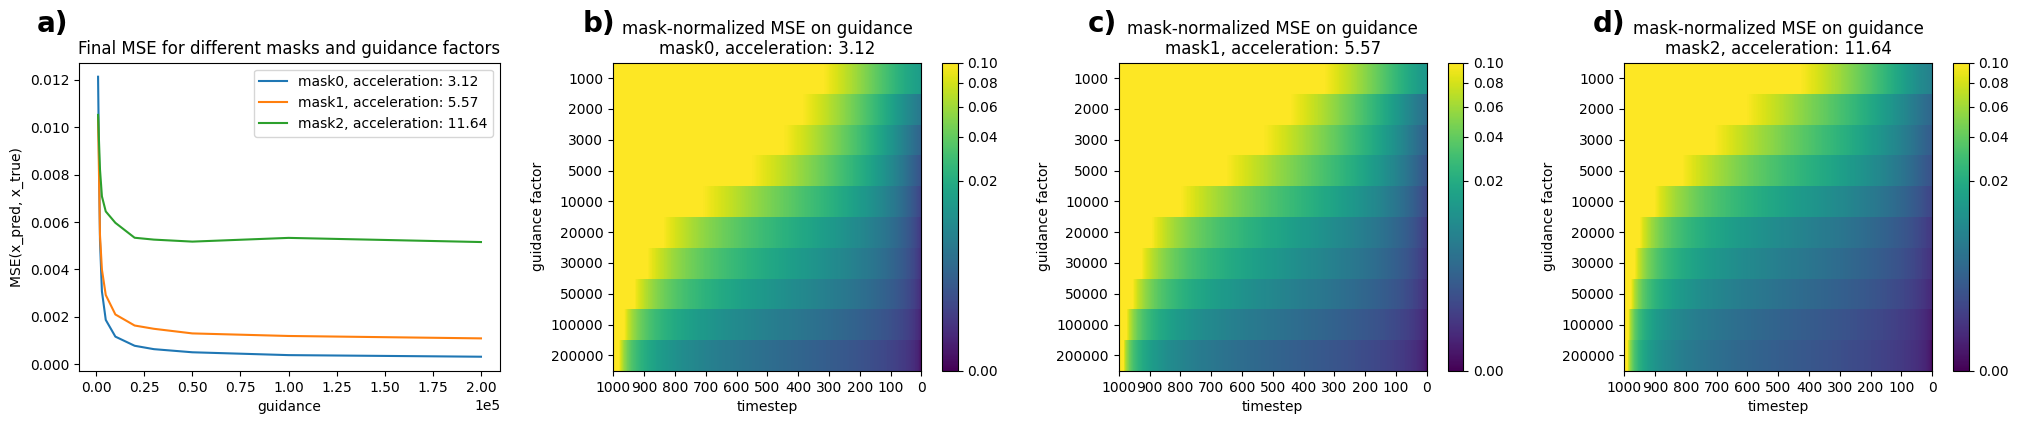
\includegraphics[width=\textwidth]{images/direct_sampling.png}
    \caption[Direct Sampling with Loss Guidance]{Results from Direct Sampling with Loss Guidance: a) Final MSE of the reconstructions for various guidance factors and accelerations. b) - d) Plots of running losses, clipped at 0.1, for various guidance factors and accelerations. Counterintuitively, losses decrease faster for higher accelerations, which is likely due to the fact that higher accelerations concentrate losses in central k-space, which is determined earlier than the outer regions.}
    \label{fig:lossguidancelosses}
\end{figure}
Plots of the gradients and of the dominant frequencies for guidance can be seen in Fig.~\ref{fig:lossgradients}. Since these gradients are very noisy, they were averaged over a batch of 1200 equal images. The spectra of the gradients show that lower frequencies indeed guide more strongly in the beginning, but contrary to the observations from section~\ref{sec:predvariance}, they do not dominate the higher frequencies, which already have significant values early on.

\subsection{Increased Computation Time for Better Reconstruction Quality}
As introduced in~\ref{sec:morecompute}, DDPMs offer several ways of using more computing resources for potentially higher sample quality. For the lower accelerations this was of minor interest since their reconstructions were never observed to suffer from artifacts and no tradeoff between data consistency and prior was ever necessary, even for very large guidance factor. For the highest acceleration, the long-grained resampling proved especially helpful, producing alias-free reconstructions of high quality for all inspected samples. This also expressed itself in a significant drop in MSE: For the direct sampling scheme, the best MSE at acceleration $\approx 11.64$ was 0.0052 at $g=200'000$ and it dropped to 0.0016 for long-grained resampling with $j=100$ and $g=20'000$. This MSE is almost in the same order as the one for direct sampling with acceleration $\approx 5.57$, which was 0.0011 at $g=20'000$. The experiment was also repeated for the lower accelerations, but their reconstructions did not profit from the additional computation time. Reconstructed samples for the highest acceleration (11.64) and several guidance factors and jump lengths can be viewed in Fig.~\ref{fig:longgrainedmask2}. The measured MSEs of the final predictions are shown in Fig.~\ref{fig:mselonggrained}.
\begin{figure}
    \centering
    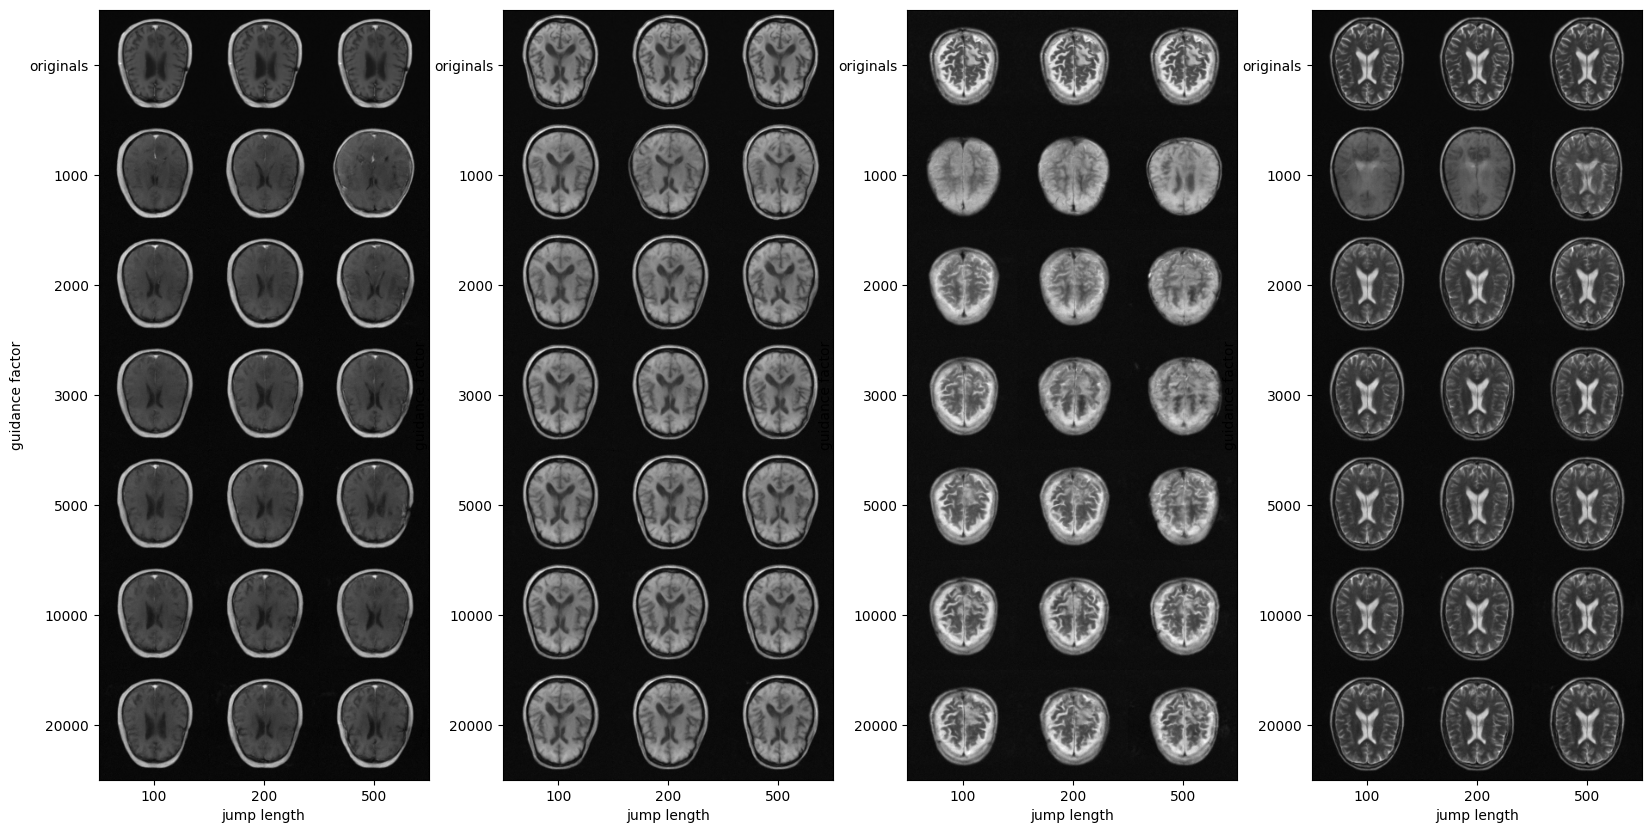
\includegraphics[width=\textwidth]{images/msk2_longRes.png}
    \caption[Comparison of Reconstruction from High Acceleration with Long-Grained Resampling]{Comparison of Reconstruction from High Acceleration with Long-Grained Resampling: Resampling has a significant impact on the reconstruction quality for the high acceleration of $\approx 11.64$ as is demonstrated by these 4 samples for several guidance factors and several jump lengths.}
    \label{fig:longgrainedmask2}
\end{figure}
\begin{figure}
    \centering
    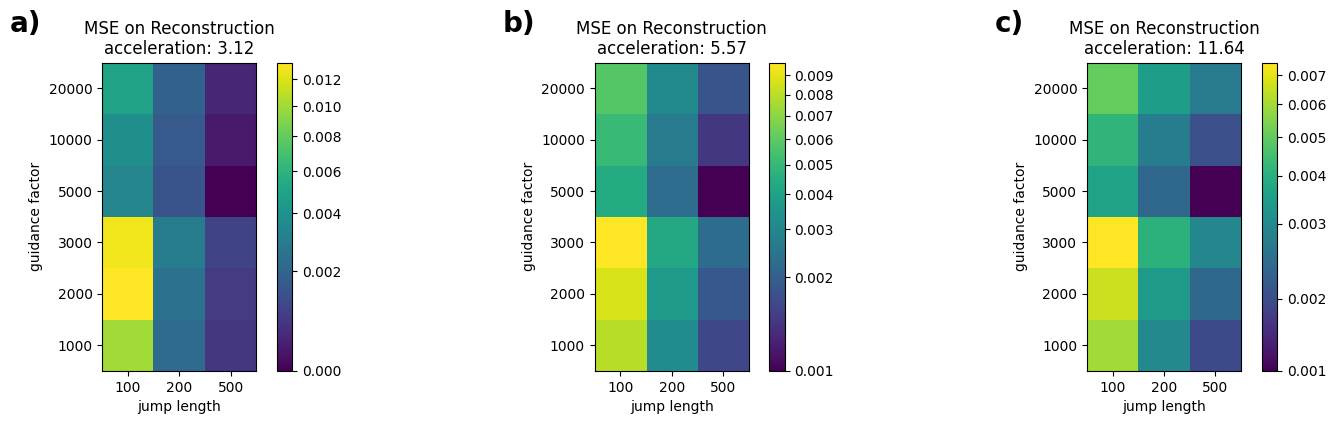
\includegraphics[width=.7\textwidth]{images/globalresamplingmse.png}
    \caption[Reconstruction MSE with Long-Grained Resampling]{a) - c) MSEs of reconstructions when using long-grained resampling for several accelerations, guidance factors and jump lengths. The values are comparable to direct sampling for the two lower accelerations, but are significantly better for the highest acceleration at $g=5000$ and $j=500$.}
    \label{fig:mselonggrained}
\end{figure}